
\documentclass{uonmathreport}


% this allows one to include .jpg etc figures using pdflatex
% change the optional argument if you use dvips or others
\usepackage[pdftex]{graphicx}

\usepackage{graphicx} %Loading the package
\graphicspath{{ParabolicPlots/}{EllipticalPlots/}{Aposteriori/}} 
%\graphicspath{EllipticalPlots/} 
\usepackage{amsthm}
\usepackage{bigints}
\usepackage{relsize}
\usepackage{amsmath}
\usepackage{tikz}
\usepackage{listings}
\lstset {backgroundcolor=\color{black!5}, basicstyle=\footnotesize, stringstyle=\color{red}, commentstyle=\color{green!50!black}, basicstyle=\footnotesize\ttfamily, keywordstyle=\color{blue}, 
}
\usepackage{xcolor}
 
\theoremstyle{definition}
\newtheorem{definition}{Definition}[section]

\theoremstyle{problem}
\newtheorem{problem}{Problem}[section]

\theoremstyle{theorem}
\newtheorem{theorem}{Theorem}[section]

\def\realnumbers{\mathbb{R}}

\DeclareMathSizes{12}{12}{10}{10}


% other packages that maybe of use include:
% hyperref, amsthm, xy, todonotes, showkeys, ...

% change to \PJS or \DIS or \HGDIS (for BSc and MPhil)
% or \MSc (for all Msc dissertations)
\MSc

% adjust the following
\title{An Adaptive Finite Element Method Approach to the Heat Equation and the Black-Scholes Equation}
\author{Thabo Miles 'Matli}
\academicyear{2017/2018}
\supervisor{Dr. Kris Van Der Zee}

% the following are irrelevant for Msc:
\assessmenttype{Review} % or Investigation
\projectcode{XX P99}

% the following are irrelevant for PJS, PJA, DIS and HG4DIS:
% Msc: change it to G1PMD and Pure Mathematics, etc ...
\msccode{G14SCD}
\msctitle{Scientific Computation}

% gives double-spacing
\linespread{1.6}
% the margins are set automatically. Do not make them smaller.

% put your own definitions and shorthands here
\newcommand{\ZZ}{\mathbb{Z}}

\begin{document}

\maketitle

\begin{abstract}
The abstract of the report goes here. The abstract should state the
topic(s) under investigation and the main results or
conclusions. Methods or approaches should be stated if this is
appropriate for the topic. The abstract should be self-contained,
concise and clear. The typical length is one paragraph.
\end{abstract}

% Table of contents
\setcounter{tocdepth}{2}  % this will list subsections, but not subsubsections
\tableofcontents 
\newpage

\section{Introduction} \label{sec:intro}

The origin of the Finite Element Method (FEM) is generally agreed to be a paper by Courant \cite{courant1943} in 1943. Though initially obscure, it gained widespread usage in engineering as computing power became more cheaply available. Since then it has become increasingly more common in the natural sciences and more recently in financial industry \cite{topper2005option}. Though the Finite Difference Method is still overwhelming used to price options the FEM is now sometimes being instead. 

Though more technical than the Finite Difference Method, under certain circumstance the FEM has stark advantages. Two notable advantages are that the FEM is simpler to use for Partial Differential Equations (PDEs) with irregular shaped domains and that there is a very well understood theory of aposteriori errors. This theory of errors, which only requires knowledge of the estimated solution, allows for the FEM to be adapted during implementation. This adaptive methodology leads to a solution where errors are guaranteed to be within certain tolerances which allows the user to analyse the effects of changing parameters. Also, adaptivity leads to a solution that should be in some sense efficient as ideally maximum accuracy achieved for the minimum degrees of freedom. This concept of efficiency is what we look to investigate further in this paper.

The pioneering work of Babuska et al \cite{babuska1981posteriori} in the 1980s showed the first examples of how an aposteriori error estimate could be used to implement adaptive FEM. The research moved quickly and attempts at adaptive mesh refinement for parabolic PDEs began towards the end of the same decade see \cite{eriksson1991adaptive}, \cite{johnson1988error} and others. Despite the research into these methods and the adoption of adaptive FEM in science and engineering there are still some theoretical results outstanding. Convergence and optimal complexity have only been shown for linear elliptical PDEs and only quite recently \cite{morin2008basic}, \cite{siebert2011convergence}. Even these recent results only show that there is convergence to a solution and do not imply an order of convergence for the adaptive methods.

The rest of this dissertation comprises:
 
...

As show by Bergam \cite{Bergam} in their article.


% this is a comment in the file that won't appear in the output

The end of the introductory section would typically outline the
structure of the report. In this template, section \ref{sec:background}
gives the background of the topic, sections \ref{sec:my1} and
\ref{sec:my2} contain the bulk of the work and section
\ref{sec:conclusions} summarises and discusses what has been
achieved. Appendix \ref{app:rawdata} displays the raw data, and
certain technical calculations for section \ref{sec:my1} are deferred
to appendix \ref{app:calculations}.

\newpage

\section{The Linear Heat Equation} \label{sec:Heat Equation}

The Heat Equation provides a simple situation within which we can understand and demonstrate the implementation of the Finite Element Method and adaptive algorithms. Conversely it is fundamental enough that it would allow someone reading this dissertation to easily build on our findings to access a different but connected problem for example the Black-Scholes equation. It can be thought of as a prototypical parabolic equation and this was our motivation for studying it.

In this section we will describe the derivation of the Heat Equation in one dimension. We will first do this in the steady state i.e. where $\frac{du}{dt}=0$ and then extend this to the time dependent equation. We do this just to refresh the reader's knowledge of the properties of the equation. 

\subsection{The Heat Equation in Steady State} \label{subsec:Steady State}

The steady state equation in one dimension can be thought of as describing a thin rod of uniform material on the interval $I =$ [0, L]. As we are only considering the one dimensional problem heat is only conducted in the $x$ direction. The rod is heated by a source $f$ which we assume to have been acting continuously for long enough to reach the steady state. 

Let $q$ be the heat flux i.e flow of energy per unit of area per unit of time and let $S$ be the cross section of the rod. As flux is a vector quantity it needs a direction and we take this as the direction of x increasing. The first law of thermodynamics on conservation of energy tells us that the flow out of the rod must equal the flow in from the heat source. Hence we have:

\begin{equation}
q(L)S(L) - q(0)S(0) =  \int_I  f  dx	\label{eq:Conservation of Energy1}
\end{equation}

We now divide both sides of \eqref{eq:Conservation of Energy1} by L and take L $\rightarrow$ 0. Hence we have the differential equation:

\begin{equation}
(Sq)' = f	\label{eq:Conservation of Energy2}
\end{equation}

Employing Fouriers law which in this context can be understood as the flux being negatively proportional to the temperature gradient:

\begin{equation}
q = kT'	\label{eq:Fouriers Law}
\end{equation}

here k represents the heat conductivity of the rod.

Together \eqref{eq:Conservation of Energy2} and \eqref{eq:Fouriers Law} give us the Heat Equation:

\begin{equation}
-(SkT')'= f 	\label{eq:Steady State Heat Equation}
\end{equation}


\subsection{The Time Dependent Problem} \label{subsec:Time Dependent Heat Equation}

The time dependent problem is very similar to the steady state form. We introduce a function e which is the energy per unit length within the rod. We use the the conservation of energy principle again but this time we use the fact that the sum of the resultant heat flux is equal to the rate of change of internal energy. Here rate of change of $e$ is denoted by $e\dot{•}$

\begin{equation}
\int_I  \dot{e} dx =   q(0)S(0) - q(L)S(L)  \int_I  f  dx	\label{eq:Conservation of Energyt1}
\end{equation}

Once again dividing by L and letting L $\rightarrow$ 0.

\begin{equation}
\dot{e} + (Sq)' = f	\label{eq:Conservation of Energyt2}
\end{equation}

Finally assuming that the energy depends linearly on the the Temperature

\begin{equation}
e = mT	\label{eq:Energy and Heat}
\end{equation}

And using \eqref{eq:Fouriers Law} and combining \eqref{eq:Conservation of Energyt1} and \eqref{eq:Conservation of Energyt2} we have the transient Heat Equation which we will refer through out the rest of this paper simply as the Heat Equation:

 \begin{equation}
m\dot{T} - (SkT')' = f	\label{eq:Heat Equation}
\end{equation}


\clearpage
\subsection{Boundary Conditions} \label{subsec:Boundary Conditions}



\begin{figure}[h]
   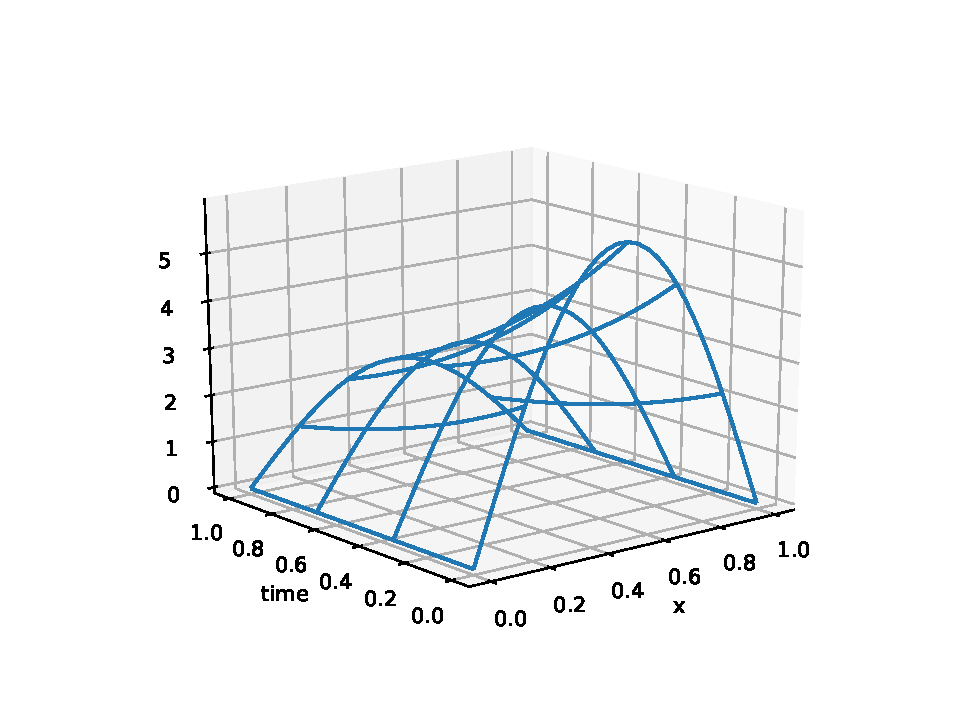
\includegraphics[width=0.5\textwidth]{Heat1.pdf}
   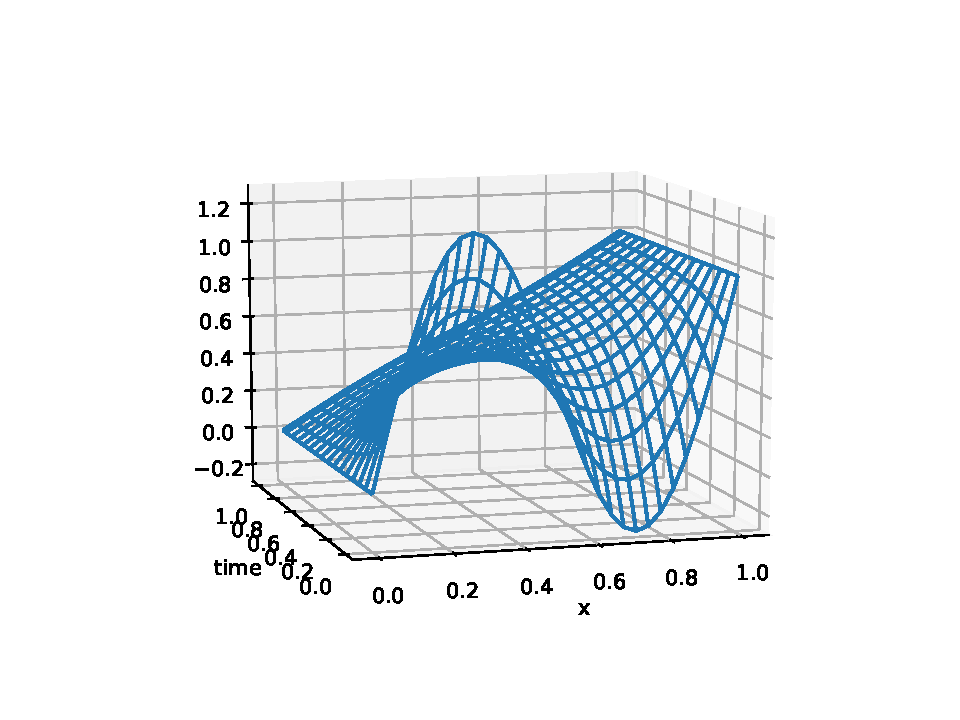
\includegraphics[width=0.5\textwidth]{Heat2.pdf}
   
 \caption{$f= 0$, $m=1$, $S = 1$, $k = \pi^-2$}
 \label{fig:Heat1}
\end{figure}



\clearpage

\section{The Finite Element Method} \label{sec:FEM}

This section is concerned with the discretisation of the Heat Equation by Finite Elements. Though not uncommon, the FEM is not necessarily widely known by the average postgraduate mathematician. As such we will provide a fairly detailed description of the method and full derivation of the scheme. A very nice introduction to the subject if more detail is needed is \cite{larson2013finite}.

The underlying practical steps to the method are:

\begin{enumerate}
\item Finding a variational form of the equation we are looking to solve. This will allow us to look for a solution which satisfies the equation in some weak sense. This step requires the introduction of the function spaces in which we can study our  equation and look for its solution. We will see that these spaces are Sobolev spaces.

\item Creating the subdivision of our domain $\Omega$.

\item Taking the variational form, which we have at first defined in an infinite dimensional function space $V$, and approximating it on a finite dimensional sub-space $V_{h}$. In our case the subspace will be piecewise polynomial functions defined on our subdivision.

\item Projecting the boundary conditions onto the finite dimensional space.
\end{enumerate}

Once the mathematical context of the Finite Element has been outlined we will move on to finding the weak formulation of the Heat Equation. With this done we will consider the finite dimensional subspace and the elements that will be used in our discretisation. We will close the chapter will a discussion of other possible choices for elements.

\subsection{Sobolev Spaces} \label{subsec:Sobolev}

We begin by stating the notation to be used in this dissertation and also stating some of the relevant definitions and results from functional analysis.

\theoremstyle{definition}
\begin{definition}{Continuous Functions}
Let $\Omega \subset \mathbb{R}^n, n \geq 1$ be an open bounded set. 
\begin{itemize}
\item We define $C(\Omega)$  the set of all real-valued and continuous functions defined on $\Omega$.
\item For $m \geq1$ we write $C^m(\Omega)$ to denote the set of m times continuously differentiable functions  i.e. that $C^m(\Omega) = \{f \in C(\Omega) : f^{(k)} \in C(\Omega)\quad \forall k \leq m\} $.
\item Let $C^{\infty}_0(\Omega) $ denote the set of all infinitely many times differentiable that vanish on the boundary of $\Omega$.
\end{itemize}
\end{definition}

\theoremstyle{definition}
\begin{definition}{$L^p$ Space}

$\|u\|_{L_2(\Omega)} := \mathlarger{\Big(\int_\Omega  { |u|^p } dx\Big)}^{\frac{1}{p}} < \infty$

\end{definition}


\theoremstyle{definition}
\begin{definition}{Multi Index}

$\alpha = (\alpha_1, \alpha_2, ... \alpha_n) \in \mathbb{N}^n \quad \quad   |\alpha| = \alpha_1 + ... \alpha_n$

Define the Multi Index 

$D^{\alpha} = \Big(\frac{\partial}{\partial x_1}\Big)^{\alpha_1}...\Big(\frac{\partial}{\partial x_n}\Big)^{\alpha_n} = $
$\frac{\partial^{|\alpha|}}{\partial x^{\alpha}_1 ... \partial x^{\alpha}_n}$

We can now generalise our earlier definition of continuous differentiable functions to an analogous idea with the multi index which will be relevant to partial differentiation.

$C^m(\Omega) = \{f \in C(\Omega) : D^\alpha f \in C(\Omega)\quad \forall |a| \leq\leq m\} $

\end{definition}


\theoremstyle{definition}
\begin{definition}{Weak Derivative}

Say $\psi_\alpha$ is a locally integrable 

$\mathlarger{\int_\Omega  \psi_\alpha(x) \cdot v(x) dx} = (-1)^{\alpha} \mathlarger{\int_\Omega  u(x) \cdot D^{\alpha} v(x) dx} \forall v \in C^\infty_0(\Omega)$

\end{definition}

\theoremstyle{definition}
\begin{definition}{Sobolev Space}

$H^{m}(\Omega) = \{ u \in L_2(\Omega) : D^{\alpha} u \in L_2(\Omega), |\alpha| \leq m \}$

$$\|u\|_{H^m(\Omega)} :=  \Big(\mathlarger{\sum_{|\alpha|\leq m}}\|D^{\alpha}u\|^2_{L_2(\Omega)} \Big)^{\frac{1}{2}} $$


\end{definition}

The Lax Milgram theorem shows shows the existence and uniqueness of a solution to the PDE. 


\begin{theorem}[Lax Milgram]
\label{Lax Milgram}
Let V be a real Hilbert Space with associated norm $\|\dot{•}\|$. Also let $a(\dot{•}, \dot{•})$ be a bilinear functional on V x V with:

(a) $a(\cdot, \cdot)$ is coercive, i.e. there exists a positive constant $c_0 \forall v \in V |a(v, v)|  \geq c_0 \|v\|^2_V$ 

(b) $a(\cdot, \cdot)$ is continuous i.e. there exists a positive constant $c_1 \forall v, w \in V |a(v, w) \leq c_1 \|v\|_V \|w\|_V$ 

and for $\ell(\cdot)$ a bilinear functional also on V such that 

(c) $\ell(\cdot)$ is continuous i.e. there exists a positive constant $c_2 \forall v \in V |\ell(\cdot)|  \leq c_2 \|v\|_V$

Then there $\exists u \in V: a(u, v) = \ell(v) \forall v \exists V$ and u is unique.
\end{theorem}

This version of the theorem is Weaker than the refinement proved by Babuska but it sufficient for our purposes. The refined theorem is available f in most textbooks on the FEM.




\clearpage

\subsection{Subdivion and basis functions} \label{subsec:Subspace}

Take the subdivision on $x \in \Omega$ in our model problem \ref{eq:Steady Diffusion1}. We subdivide the domain into N intervals $[x_k, x_{k+1}] \quad k=0, 1, ... , N-1$. This subdivision may not be regular and when later in this dissertation we begin seeking an adaptive solution will very rarely be regular. intervals may be referred to as elements and give the FEM its name.
\\
\\

\begin{center}
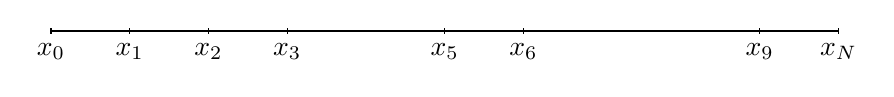
\begin{tikzpicture}

\draw[thick] (0,0) -- (10,0) node[anchor=north west] {};
\foreach \x in {0,1,2,3,5,6,9}
   \draw (\x cm,1pt) -- (\x cm,-1pt) node[anchor=north] {$x_\x$};

\draw (10 cm,1pt) -- (10 cm,-1pt) node[anchor=north] {$x_N$};

\end{tikzpicture}
\end{center}


We now define the FEM basis function on this grid. 

\begin{equation}
\phi_j(x) =  \Big(\:1 - \Big|\frac{x-x_k}{h_i}\Big| \: \Big)_+ , \quad j = 0,1,..., N
\end{equation}





\subsection{The Weak Formulation} \label{subsec:Weak Formulation}

Now we have defined the mathematical context let us solve a problem via the FEM. Take the stationary heat equation.

\begin{subequations} 
\label{eq:Steady Diffusion1} 
\begin{align}
-u'' &= f		\quad \quad  x \in [0, 1] \\  	
u(0) &= 0 \\
u(1) &= 0
\end{align}
\end{subequations}

The first step of solving this and any PDE by the FEM is to find a suitable weak formulation. This is given by multiplying both sides of the equation by a test function in the Sobolev space $v \in H^1_0(0, L)$.

\begin{equation*}
\int_0^L  u'' v  dx = \int_0^L  f v dx 	\quad \quad  dx \forall v \in H^1_0(0, L)
\end{equation*}

Integrating by parts on the left leads us to our weak formulation of \ref{eq:Steady Diffusion1}

\begin{problem}{Weak Formulation} \label{prob:Weak Formulation Elliptic}
\\Find $\quad u \in H^1_0(0, 1)$:
\begin{align*}
\int_0^L  u' v'  dx =   \int_0^L  f v dx  \quad \quad  \forall v \in H^1_0(0, L)
\end{align*}
$\forall v \in H^1_0(0, L)$
\end{problem}

Define 
\begin{equation*}
\int_0^L  u' v'  dx = a(u, v)  	
\int_0^L  f v dx  =  \ell(v)
\end{equation*}

This gives us the linear and bilinear form with can be used to show by \ref{Lax Milgram} that $u$ exists and is unique. However, our test function has been chosen simply some function in the Sobolev space which has infinitely many functions defined within it and is described as infinite dimensional. 

To find the FEM approximation to \ref{Steady Diffusion1} we look for a solution in a finite dimensional subspace of $V\subset H^1(0, L) $. The subspace we chose consists of continuous piecewise linear functions of defined on some given subdivision of $\Omega$. Then we can restate the weak formulation by the following:

\begin{problem}{FEM Approximation} \label{prob:Approx1}\\
Find $\quad u_h \in  V\subset H^1(0, 1) \quad : \quad a(u_h, v_h) =  \ell(v_h) \quad \forall v_h \subset V.$
\end{problem}

We now define a basis for our domain 
As we are looking to approximate u by a piecewise linear function $u_h$ 

Let the subspace $V$ have dimension $N(h)$ and $V = span\{\phi_1, ..., \phi_{N(h)}\}$. Hence, we have defined our subspace by linearly independent basis functions $\phi_i$.

Now we can define our approximation $u_h$ to \ref{eq:Steady Diffusion1} by:

\begin{equation*}
u_h(x) = \sum_{j=1}^{N(h)} U_j \cdot \phi_h(x)
\end{equation*}

With $U_j \: j = 1, ..., N(h)$ being constants to be determined. We can now rewrite \ref{prob:Approx1} by the following:

\begin{problem}
$$\sum_{j=1}^{N(h)}U_j \: a( \,\phi_j(x),\, \phi_i(x)) = \ell(\,\phi_i(x)\,) $$
\end{problem}

This gives a system of linear equations with $a( \,\phi_j(x),\, \phi_i(x))$ an $N(h)\times N(h)$ matrix. To form and solve this system we need to introduce the FEM basis function 

\begin{subequations} 
\begin{align}
A_{ij} =& \int_I \phi_i \phi_j dx \label{eq:stiff}\\
b_i =& \int_I  \, f\phi_i dx
\end{align}
\end{subequations}

\begin{equation}
AU = F			\label{eq:system1}
\end{equation}

\subsection{Results} \label{subsec:results1}

\begin{figure}[h]
   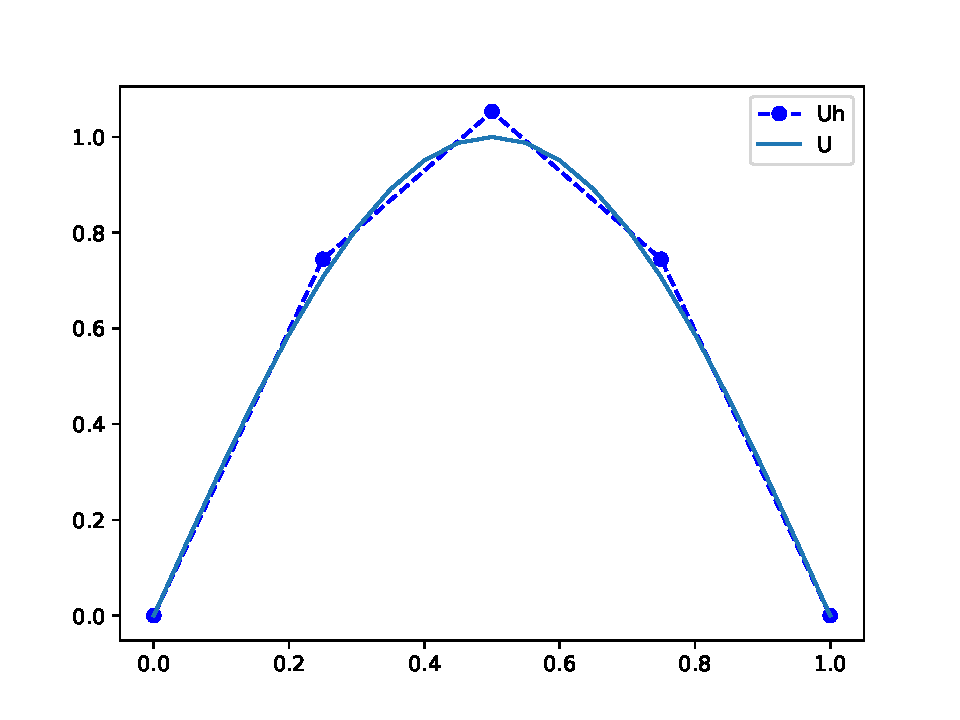
\includegraphics[width=0.5\textwidth]{EllipticPDE2.pdf}
   
 \label{fig:eliptic1}
\end{figure}

\begin{center}
  \begin{tabular}{r|cccccc}
    $Mesh$   & h & $\|u-u_h\|_{L_2(0,1)}$ & s & $\|u-u_h\|_{H^1(0,1)}$ & s  \\ \hline
    $1$ & $\tfrac{1}{4}$ & 0.0174706 & 2 & 0.511854 & 5  \\
    $2$ & $\tfrac{1}{8}$ & 0.00413879 & 5 & 0.252837 & 11  \\
    $3$ & $\tfrac{1}{16}$ & 0.00102063 & 5 & 0.12604 & 11  \\
	$4$ & $\tfrac{1}{32}$ & 0.000254283 & 2 & 0.0629727 & 5 \\
    $5$ & $\tfrac{1}{64}$ & 6.3516e-005 & 5 & 0.0314805 & 11  \\
    $6$ & $\tfrac{1}{128}$ & 1.58756e-005 & 5 & 0.0157395 & 11 \\
  \end{tabular}
\end{center}




\begin{figure}[h]
   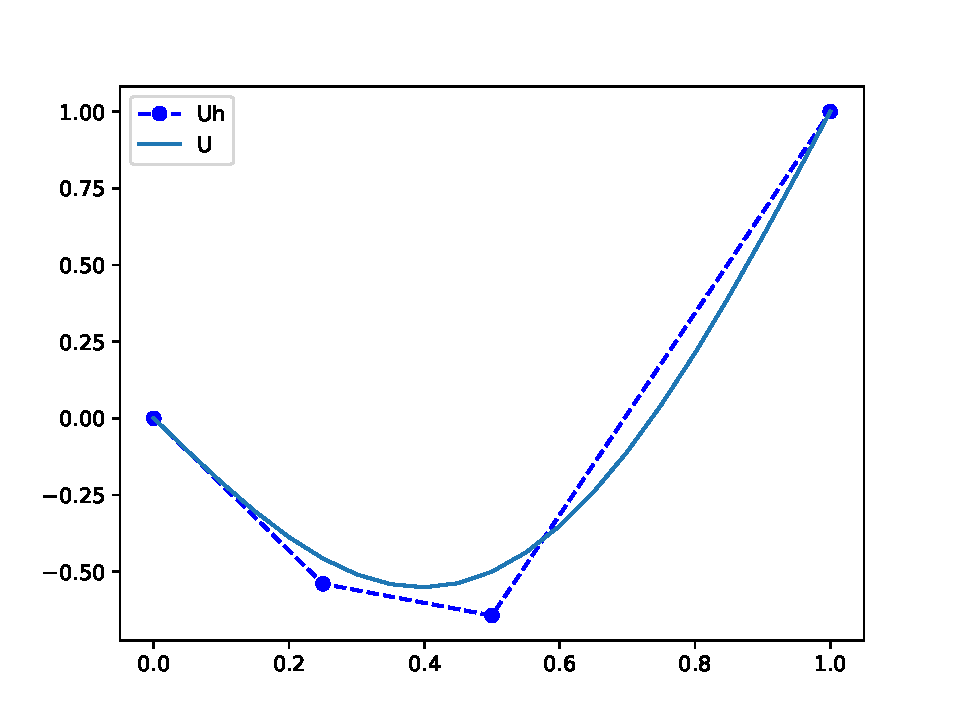
\includegraphics[width=0.5\textwidth]{EllipticPDE1_hi.pdf}
   
 \label{fig:eliptic1}
\end{figure}

\begin{center}
  \begin{tabular}{r|cccccc}
    $Mesh$   & DOGs & $\|u-u_h\|_{L_2(0,1)}$  & $\|u-u_h\|_{H^1(0,1)}$   \\ \hline
    $1$ & $4$ & 0.0776354  & 0.825144   \\
    $2$ & $7$ & 0.0170398  & 0.40185   \\
    $3$ & $13$ & 0.00411272  & 0.199548   \\
	$4$ & $25$ & 0.00101902  & 0.0996014 \\
    $5$ & $49$ & 0.000254182  & 0.0497791   \\
    $6$ & $97$ & 6.35097e-005  & 0.0248868  \\
  \end{tabular}
\end{center}

\begin{figure}[h]
   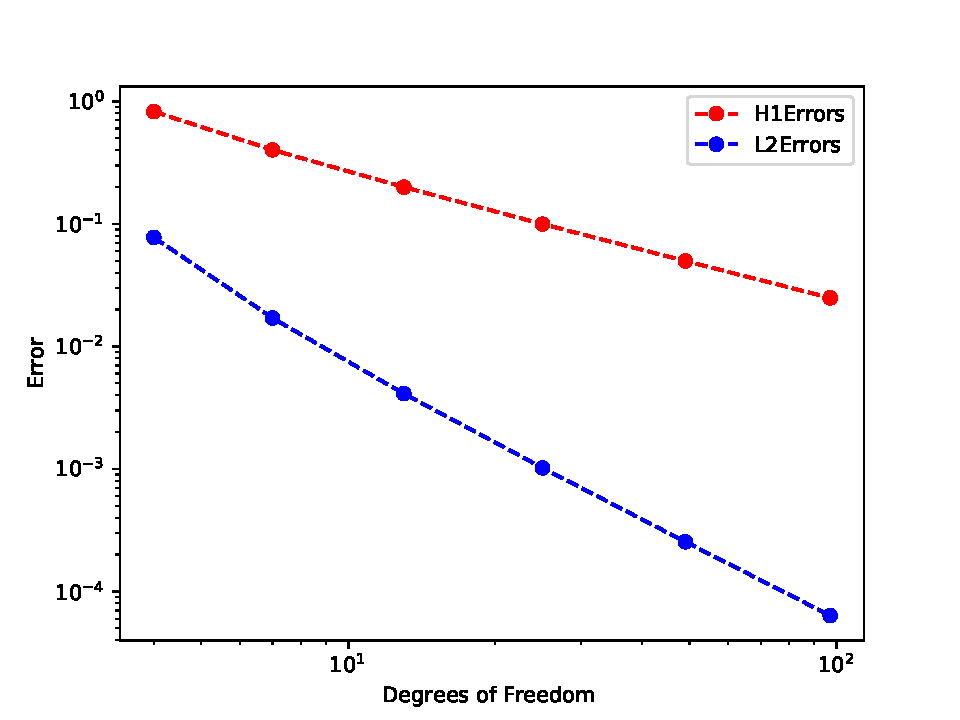
\includegraphics[width=0.5\textwidth]{EllipticPDE1Convergences.pdf}
     
 \label{fig:eliptic1}
\end{figure}

\subsection{Implementation} \label{subsec:Implementation1}

It is evident that all the matrices that arise from the one dimensional FEM are tridiagonal. This is important as there are efficient algorithms available for solving tridiagonal systems. To store the matrix we only need to  none zero arrays that compose it. This is an ideal opportunity to create a data structure to store these matrices and also to make use of some object oriented design patterns to associate the characteristics of the matrices to a special case of tridiagonal matrices such as \ref{eq:stiff}. One possible declaration is given below:

\begin{lstlisting}[language=C++]
class TriDiagMatrix{
public:
    void SetMatrix( std::vector<double> Diagonal,
         std::vector<double> LowerDiag, std::vector<double> UpperDiag);

    void MatrixSolver( std::vector<double> f,
         std::vector<double> &x );

protected:
    std::vector<double> mpDiagonal;
    std::vector<double> mpLowerDiag;
    std::vector<double> mpUpperDiag;
};
\end{lstlisting}



The obvious advantage of a similar declaration is not only the efficiency of the storage and the methods but also the readability, polymorphism and the ease with which the code can then be tested. Once module tests have been run and effectiveness established we can derived any specific matrices we need from the above interface. The first derivation we make is for \ref{eq:stiff} also called the Stiffness matrix. This class reads a specific subdivision of the domain $\omega$ and sets the Stiffness matrix accordingly.

\begin{lstlisting}[language=C++]
class StiffnessMatrix: public TriDiagMatrix{
public:
    void BuildStiffnessMatrix ( SpaceMesh& smesh ); };

\end{lstlisting}

We are now ready to solve \ref{eq:system1}. We can now write a solve method which is as simple as the simplest psuedo-code. Called for \ref{eq:Steady Diffusion1} with  $f=\pi^2cos(\pi x - \frac{\pi}{2})$, subdivision of $\Omega$ so that $h_i = 0.25 i=1, 2, 3, 4$   the code produces the below result.\\

\begin{lstlisting}[language=C++]
void StationaryHeatEquation(){
StiffnessMatrix ( mpsmesh );
buildfvec( SpaceMesh& a_smesh, double(*f)(double))
stiff.MatrixSolver( f_vec, U );
PrintVector(U);
}
\end{lstlisting}

\clearpage

We have not yet discussed the implementation of boundary conditions. In the derivation of the weak formulation the boundary conditions are projected into the solution space. This has been done in \ref{prob:Weak Formulation Elliptic} by choosing $H^1_0(0, L)$ for our zero dirichlet boundaries.

In practise one of the major advantages of the FEM is the ease with which more complicated boundary conditions can be implemented. A detailed account of doing this in a general is given in \cite{larson2013finite}. The method they advocate is implementing Robin boundary conditions and using parameters to set Neuman conditions or approximate dirichlet conditions. From here onward this is the method used in the code from here on.



\section{The Time Dependent Problem} \label{sec:Time dependent}

Now that we have built some foundations by solving the elliptical PDE ref{eq:Steady Diffusion1} we can use the same method to discretise the space dimension of the Heat Equation.
\begin{subequations} 
\begin{align}
  \dot{u} - u'' = & f \quad x \in [0, L], \quad t \in (0, T]  \\ \label{eq:Simple Heat}
  u(0, t) & = u(L, t) = 0\\
  u(x, 0) & = u_0(x)   
\end{align}
\end{subequations}

Multplying $\dot{u} - u'' = f$ by a test function  $v \in H^1_0(0, L)$  on both sides gives:

\begin{equation*}
  \int_0^L \dot{u} v dx  - \int_0^L  u'' v  dx =   \int_0^L  f v  dx   
\end{equation*}

Integrating by parts yields:

\begin{equation*}
  \int_0^L \dot{u} v dx  + \int_0^L  u'' v  +u(0)v(0) - u(L)v(L) dx =   \int_0^L  f v  dx   
\end{equation*}

\begin{equation*}
  \int_0^L \dot{u} v dx +  \int_0^L  u' v'  dx =   \int_0^L  f v  dx    
\end{equation*}

The weak formulation of our problem is now given by:

\begin{problem}{Weak Formulation} \label{weak2}
Find $\quad u(\cdot, t) \in H^1_0(0, L)$:
\begin{align*}
	(&\dot{u}(\cdot, t), v) + a(u(\cdot, t), v) = (f(\cdot, t), v)\\
	(&u(\cdot, 0), v) = (u_0, v)
\end{align*}
$\forall v \in H^1_0(0, L)$
\end{problem}
Here,
\begin{align*}
 a(w, v)  = \int_0^L  w' v'  dx 
 (w, v) = \int_0^L  w v  dx 
\end{align*}


To find our approximation define a mesh on $\bar{\Omega}^{\Delta t}_h =[0, 1] \times [0, T]$.\\

\begin{center}
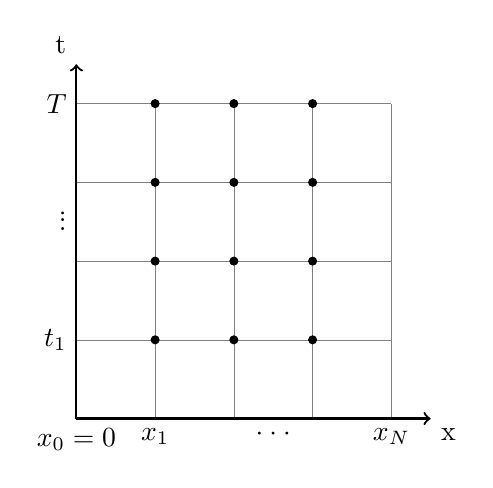
\begin{tikzpicture}

\draw[step=1cm,gray,very thin] (0,0) grid (4,4);
\foreach \x in {1,2,3}
	\foreach \y in {1, 2, 3, 4}
    	\filldraw (\x,\y) circle (0.05cm);
    	
\draw[thick,->] (0,0) -- (4.5,0) node[anchor=north west] {x};
\draw[thick,->] (0,0) -- (0,4.5) node[anchor=south east] {t};
    	
\draw (0,4) node[anchor=east] {$T$};
\draw (0,0) node[anchor=north] {$x_0=0$};
\draw (1,0) node[anchor=north] {$x_1$};
\draw (2.5,0) node[anchor=north] {$\cdot \cdot  \cdot$};
\draw (4,0) node[anchor=north] {$x_N$};
\draw (0,1) node[anchor=east] {$t_1$};
\draw (0,2.5) node[anchor=east] {$\dot{:}$};

\end{tikzpicture}
\end{center}

Let the partition on the space mesh be $0 = x_0< x_1< ...< x_N = 1$ with intervals\\ $h_i = x_i - x_{i-1}$. Let the time partition be $0 = t_0< t_1< ...< t_M = T$ time steps $\Delta t_j = t_j - t_{j-1}$. For both space and time we allow the intervals to vary.

Let $V\subset H^1_0(0, 1)$ denote the set of all continuous piecewise linear functions defined on the space mesh that are zero on the boundaries $x=0 and x=1$. 

\subsubsection{Implicit Euler} \label{subsubsec:Implicit Euler}

\ref{weak2} is the a space discrete problem, sometimes referred to as the semi-discreet problem but we now need to discretise in time to be able to find an approximation to the solution. We will use Finite Differences to discretise in time and we will choose the Implicit Euler method. 


\begin{problem}{Implict Euler Method} \label{eq:Implicit Euler}
\\Find $u_h^{m+1} \in V \quad 0 \leq m \leq M-1$
\begin{align*}
\Big(\frac{u_h^{m+1} \, - \, u_h^{m}}{\Delta t}, v_h \Big) +\: a(u_h^m, v_h) \quad=&\quad (f(\cdot, t^m), v_h) \\
(u^{0}_h - u_0, v_h)\quad  =& \quad0 \quad \forall v_h \in V
\end{align*}
\end{problem}
%a(u_h^m, v_h) =& (f(\cdot, t^m), v_h) \\
%{u^{0}_h - u_0, v_h) =& 0 \quad \forall v_h \in V

We can therefore rewrite the system as:

\begin{align*}
( u_h^{m+1} \, v_h)  + \: \Delta t a(u_h^m, v_h) \quad=\quad (u_h^{m}, \, v_h ) \:+\: \Delta t(f(\cdot, t^m), v_h) \\
v_h \quad \forall v_h \in V \quad 0 \leq m \leq M-1 \\
\end{align*}
with
\begin{equation}
(u^{0}_h) \quad  = \quad u_0, v_h \quad \forall v_h \in V
\end{equation}

\subsection{Results} \label{subsec:results2}


\begin{figure}[h]
   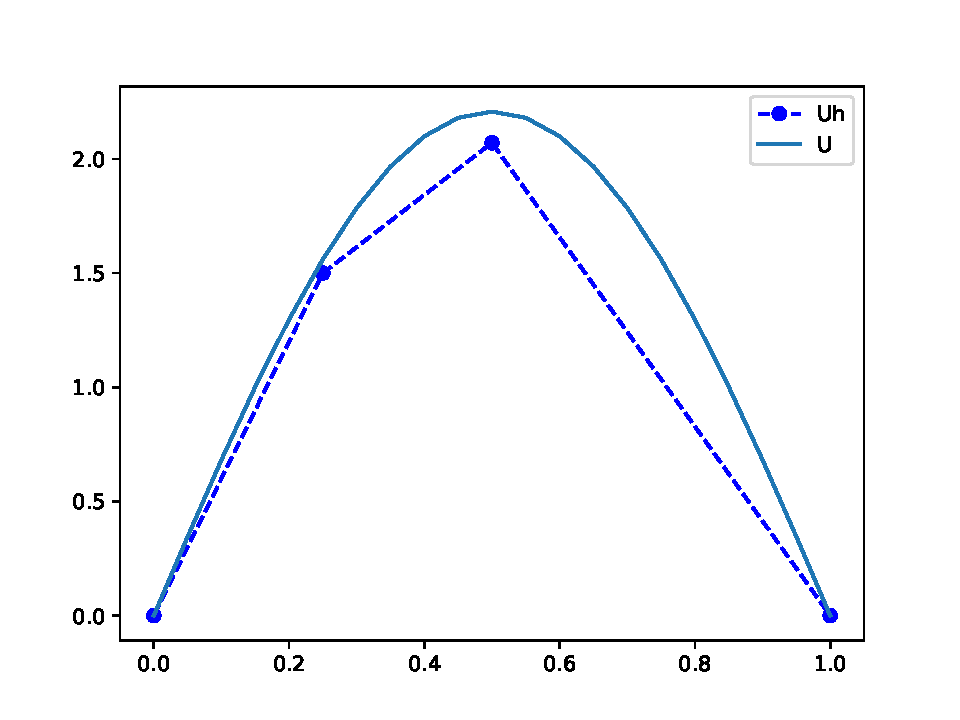
\includegraphics[width=0.5\textwidth]{OriginalPDEcoarse.pdf}
   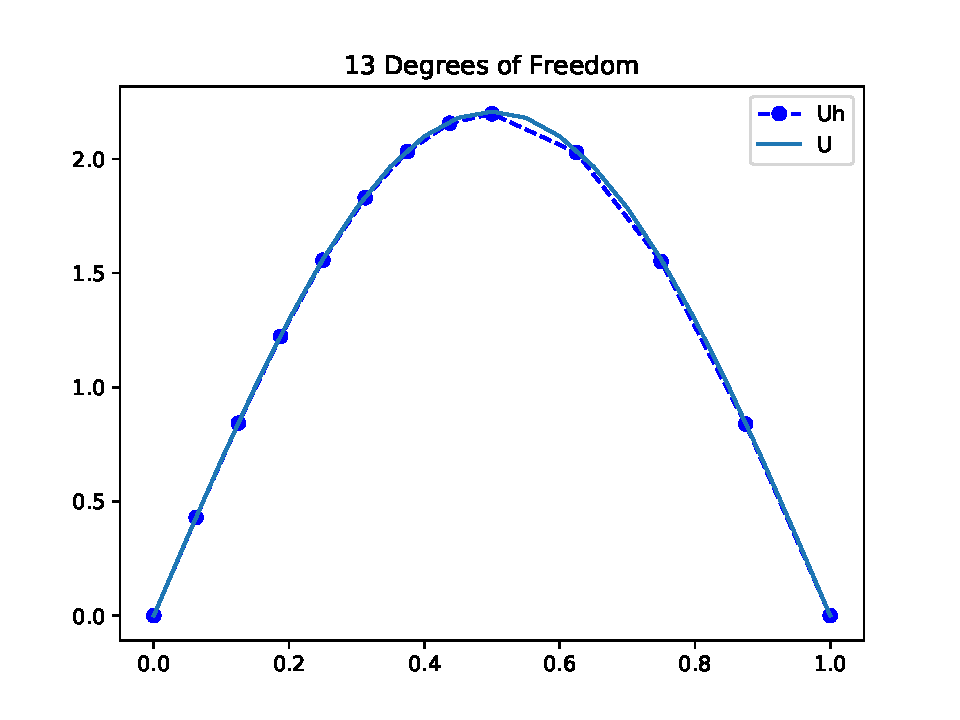
\includegraphics[width=0.5\textwidth]{OriginalPDEfine.pdf}
   
 \label{fig:OriginalPDEcoarse}
\end{figure}



\begin{figure}[h]
   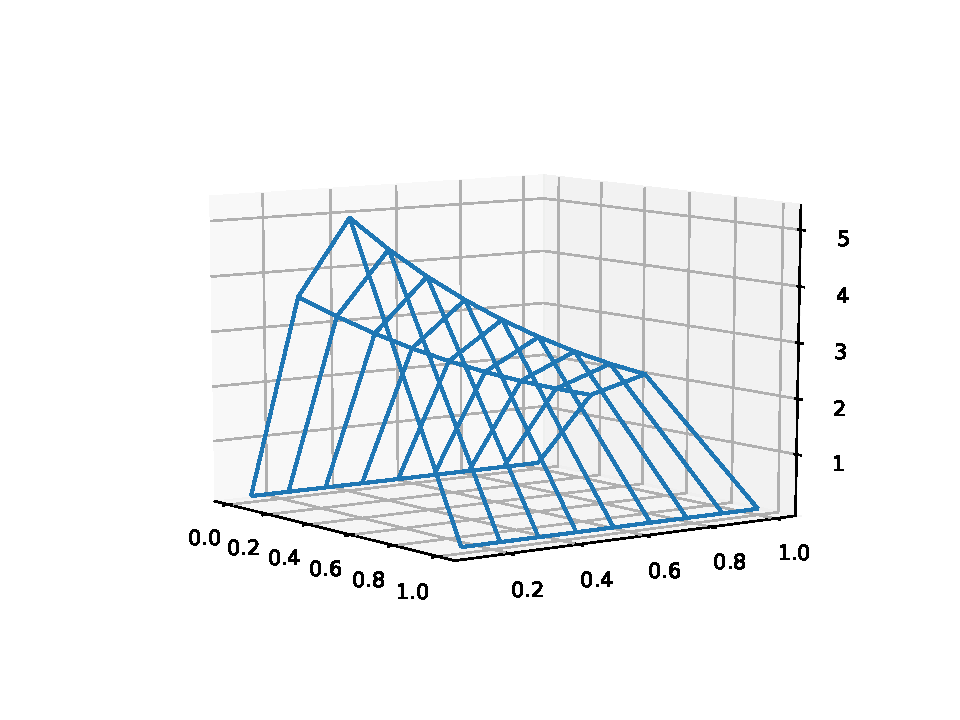
\includegraphics[width=0.5\textwidth]{firstPDE3d.pdf}
   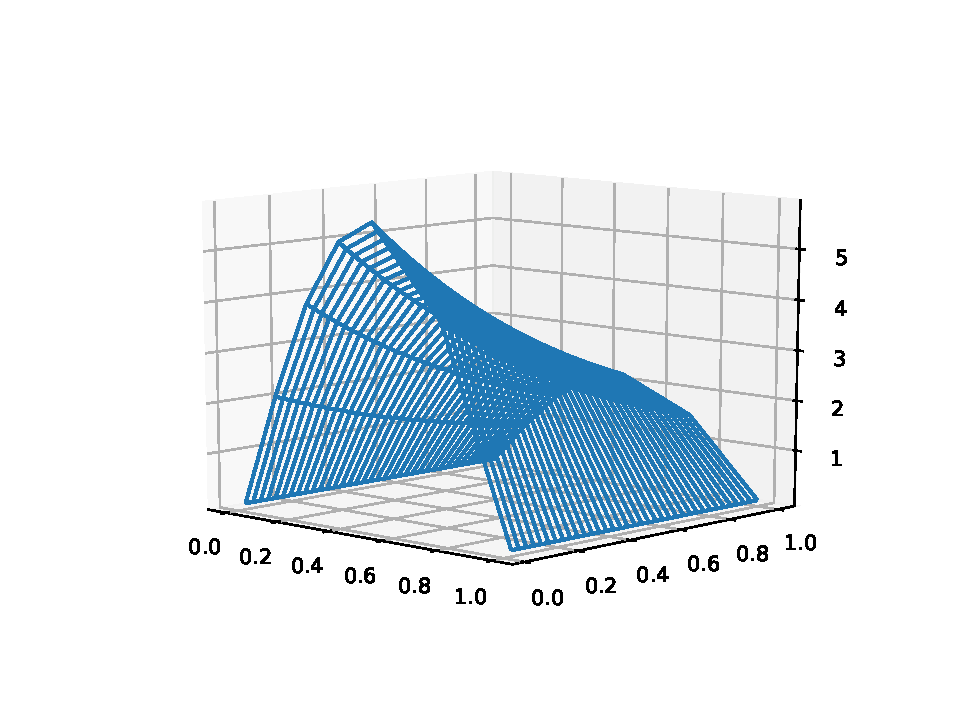
\includegraphics[width=0.5\textwidth]{firstPDE3dfine.pdf}
   
 \label{fig:firstPDE3d}
\end{figure}


\begin{figure}[h]
   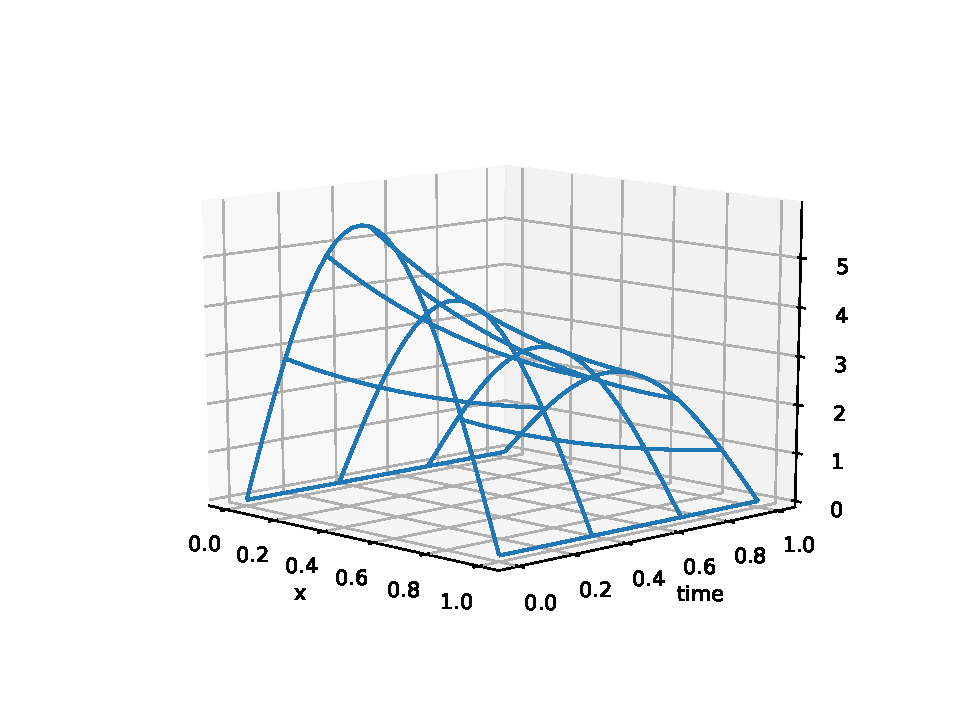
\includegraphics[width=0.5\textwidth]{Heat1angle.pdf}
   
 \label{fig:Heat1}
\end{figure}



\begin{center}
  \begin{tabular}{r|cccccc}  \label{table:Parabolic1}
    $Mesh$   & DOGs & $\|u-u_h\|_{L_2(0,1)}$ & s & $\|u-u_h\|_{H^1(0,1)}$ & s  \\ \hline
    $1$ & $4$ & 0.304466 & 2 & 1.74657 & 5  \\
    $2$ & $7$ & 0.0918245 & 5 & 0.883062 & 11  \\
    $3$ & $13$ & 0.0231464 & 5 & 0.439949 & 11  \\
	$4$ & $25$ & 0.00575675 & 2 & 0.219779 & 5 \\
    $5$ & $49$ & 0.00143142 & 5 & 0.109867 & 11  \\
    $6$ & $97$ & 0.000356574 & 5 & 0.054931 & 11 \\
  \end{tabular}
\end{center}

\begin{figure}[h]
   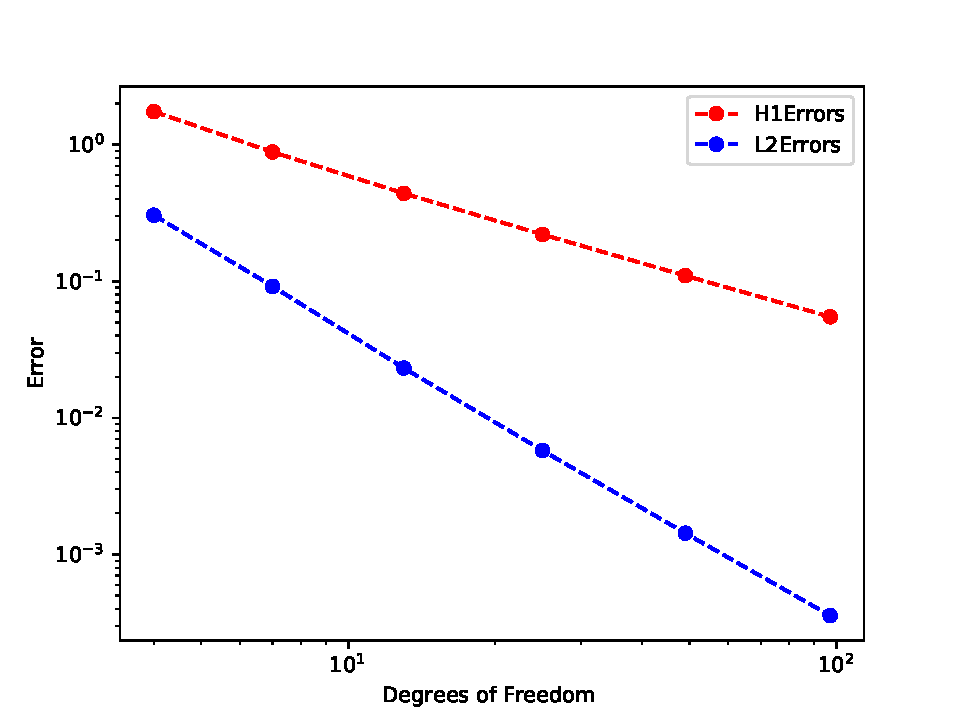
\includegraphics[width=0.5\textwidth]{ParabolicConvergencesOriginal.pdf}
   
 \label{fig:paraconvergences1}
\end{figure}






\subsection{Impementation} \label{subsubsec:Implementation}

When it comes to the computer implementation of the FEM on time dependent or multidimensional problems "meshing" is the important art-form. There are entire software packages available to carry out the creation and manipulation of mesh structures and it would therefore benefit any FEM project to either design there own data-structures or implement an existing mesh package. 

An important question when designing the data-structure and class inheritance structure is the relationship between the time-steps and the space nodes. When using Finite Difference Methods to discretise the time element the space nodes are free to vary at at a given time step however the time steps are the same when considered from a given node. This seems to both invite and discourage the creation of a single data-structure to handle meshing in both space and time. Much of the functionality of each is shared but much differs:

\begin{lstlisting}[language=C++]
class SpaceMesh
{
public:
    void CopySpaceMesh (const SpaceMesh& oldSpaceMesh);
    void BisectIntervals (std::vector<int> &intervalsForBisection);
    int meshsize();

    void CommonMesh( SpaceMesh& firstmesh, SpaceMesh& secondmesh );
    double TestFunctions(int nodeIndex, double x);
    bool Contained (double my_var );

protected:
    std::vector<double> mpSpaceNodes ;
    std::vector<double> mpSpaceMesh;
    int mpmeshsize;
};

class TimeMesh
{
public:
    void CopyTimeMesh (const TimeMesh& oldTimeMesh);
    void GenerateTimeMesh ( std::vector<double> TimeNodes );
    void BisectInterval (int lowerIndex, int upperIndex);
    int NumberOfTimeSteps();
protected:
    int mpnumberOfTimeSteps;
    std::vector<double> mpTimeNodes;
    std::vector<double> mpTimeMesh;
};


\end{lstlisting}

The question of how to structure inheritance in FEM meshes is in this case restricted to the one dimension and may seem abstract at the beginning of a project. However, there are many utility style functions i.e. adding a node or copy construction which could be simplified if there was an abstraction which could be justified rigorously. The danger of a heuristic abstraction pattern is that one of the child classes have access to a function which is not truly polymorphic and it cannot be used safely or that the program not scale because of restrictions on the inheritance. We leave the question of whether there is a rigorous way to argue for a shared parent class for a space and time meshes open. 

\newpage

\section{A Posteriori Error Analysis} \label{sec:Errors}

When a continuous problem such as the Heat Equation is discretised Finite Element Methods and solved numerically an error is incurred. Some knowledge about the error is available in advance of the implementation of a specific FEM approximation. This type of error analysis, so called a priori, is valuable for the analysis of convergence and other proofs that may be important about an FEM scheme in general. Although useful in these applications it is rare that an a priori error estimate accurately quantifies the error present in a numerical solution. As such in a practical context the a priori error cannot be used to indicate the quality of a solution. 

In contrast, a posteriori error analysis uses the computed numerical solution itself to analyses the error. Where a posteriori error estimates are available and accurate this has the obvious advantage that it describes the error in the approximation without the need for an analytical solution. This replaces the heuristics and guess work that had previously guided the error analysis of the FEM approximation in settings where no analytical solution was available. 

Since the initial pioneering methods of Babuska \cite{babuska1978posteriori} \cite{babuska1981posteriori} in this field many a posteriori error methods have been presented. Many of these have been shown to be effective in context. The emphasis in the literature has moved now from the discovery of new a posteriori estimates to the testing of the limitations of existing a posteriori estimates. All this is done primarily with the goal of validating the extensively used self-adapting FEM packages.

\subsubsection{Gradient Recovery} \label{subsubsec:KK}

The FEM provides an approximation to an unknown function, however the gradient of the function may also be of particular interest also. The gradient in the approximation is discontinuous over element boundaries but can be smoothed out by post-processing. In fact under certain circumstances the smoothed gradient is closer to the gradient of the true solution \cite{ainsworth65001posteriori}. This leads fairly directly one of the simpler a posteriori error estimates which is measuring the gradient before and after this post-processing.

Consider again the steady state one dimensional Heat Equation with conductivity co-efficient of one \ref{eq:Steady Diffusion1} and here restating its weak formulation for ease.

\begin{problem}{Weak Formulation}

Find $\quad u \in H^1_0(0, 1)$:
\begin{align*}
\int_0^L  u' v'  dx =   \int_0^L  f v dx  \quad \quad  dx \forall v \in H^1_0(0, L)
\end{align*}
$\forall v \in H^1_0(0, L)$
\end{problem}

With
\begin{equation*}
\int_0^L  u' v'  dx = a(u, v)  	
\end{equation*}

It is clear that the bilinear form is symmetric i.e.  a(w, v) = a(v, w) and it can be shown that it is coercive as described in the Lax Milgram theorem \ref{Lax Milgram}. Hence, $a(w, v)$ is an inner product on $H^1_0(0, L) (w, v)_a$.

We can then define the associated energy norm.

\begin{equation}
\|w\|_a = |(w, w)_a|^\frac{1}{2}
\end{equation}

If we measure the true error in the energy norm we get.

\begin{equation}
\|u-u_h\|_a^2 = \int_0^L  u' - u_h'  dx
\end{equation}

Which is the $L_2$ norm of of the difference between the gradient .

If we had the true gradient we would now be able to measure the true error in the energy norm. As that is unavailable we will use an estimate of the true gradient which will be obtained by some suitable post- processing of the FEM approximation to the solution. Let the post processed FEM approximated gradient be denoted by $G_h(u_h)$ then the error indicator for \ref{eq:Steady Diffusion} is given by:

\begin{equation}
\eta^2 = \int_0^L  |G_h(u_h) - u_h|^2  dx
\end{equation}

Clearly there are as many different error indicators as there are ways of processing the FEM approximation to the gradient.

Consider an FEM approximation to an PDE of form \ref{eq:Simple Heat} at an arbitrary time step.

\begin{center}
\begin{tikzpicture}

\draw[thick,->] (0,0) -- (10,0);
\draw[thick,->] (0,0) -- (0,2.5);

\draw[blue,thick,dashed] (0,0) -- (2,2.2) -- (4,2.8) -- (8,0);

\end{tikzpicture}
\end{center}

The gradient of this approximation is a discontinuous step-like function, undefined at the nodes of the space mesh.

\begin{center}
\begin{tikzpicture}

\draw[thick,->] (0,2) -- (8,2) ;
\draw[thick,->] (0,0) -- (0,6) ;

\draw[blue,thick] (0,3.1) -- (2,3.1);
\draw[blue,thick] (2,2.3) -- (4,2.3);
\draw[blue,thick] (4,1.3) -- (8,1.3);

\filldraw (2,2.7) circle (2pt);
\filldraw (4,1.8) circle (2pt);


\end{tikzpicture}
\end{center}

Intuitively a better approximation would be given by a function defined in the whole domain. A simple but logical one to use could be a continuous piecewise linear function as we have the architecture in our code to linearly interpolate sets of points. We take the midpoint of the FEM approximated gradient where currently our gradient is undefined and hence where we expect post-processing to have the greatest effect. 

More formally results exist to support this choice. In the case of a uniform partition the "super-convergence" of the centroid of two elements is shown by \cite{zlamal1978superconvergence}. Though true "super-convergence" may not be assured on our more general partition our method none-the-less should be an improvement on the untreated gradient. 

A we also need to decide what to do with the elements at each side as our current method will not produce points for on the boundaries. We will choose to have the interpolant take the value of the gradient in the centre of the elements.



\begin{center}
\begin{tikzpicture}

\draw[thick,->] (0,2) -- (8,2) ;
\draw[thick,->] (0,0) -- (0,6) ;

\draw[blue,thick] (0,3.1) -- (2,3.1);
\draw[blue,thick] (2,2.3) -- (4,2.3);
\draw[blue,thick] (4,1.3) -- (8,1.3);

\filldraw (1,3.1) circle (2pt);
\filldraw (2,2.7) circle (2pt);
\filldraw (4,1.8) circle (2pt);
\filldraw (6,1.3) circle (2pt);

\draw[blue,thick,dashed] (0,3.5) --(1,3.1) --(2,2.7) -- (4,1.8)  -- (6,1.3) -- (8,0.8);


\end{tikzpicture}
\end{center}

\subsection{Results} \label{subsec:results3}


\begin{center}
  \begin{tabular}{r|cccccc}  \label{table:IndicatorPDE1}
    $Mesh$   & DOGs & $\|u-u_h\|_{a(0,1)}$ & $\|\eta\|$  \\ \hline
    $1$ & $4$ & 1.63002 &  1.71983   \\
    $2$ & $7$ & 0.862629 &  0.878275   \\
    $3$ & $13$ & 0.435436 & 0.43934   \\
	$4$ & $25$ & 0.218313 &  0.219703  \\
    $5$ & $49$ & 0.109433 &  0.109858   \\
    $6$ & $97$ & 0.0548128 &  0.0549298  \\
  \end{tabular}
\end{center}


\begin{figure}[h]
   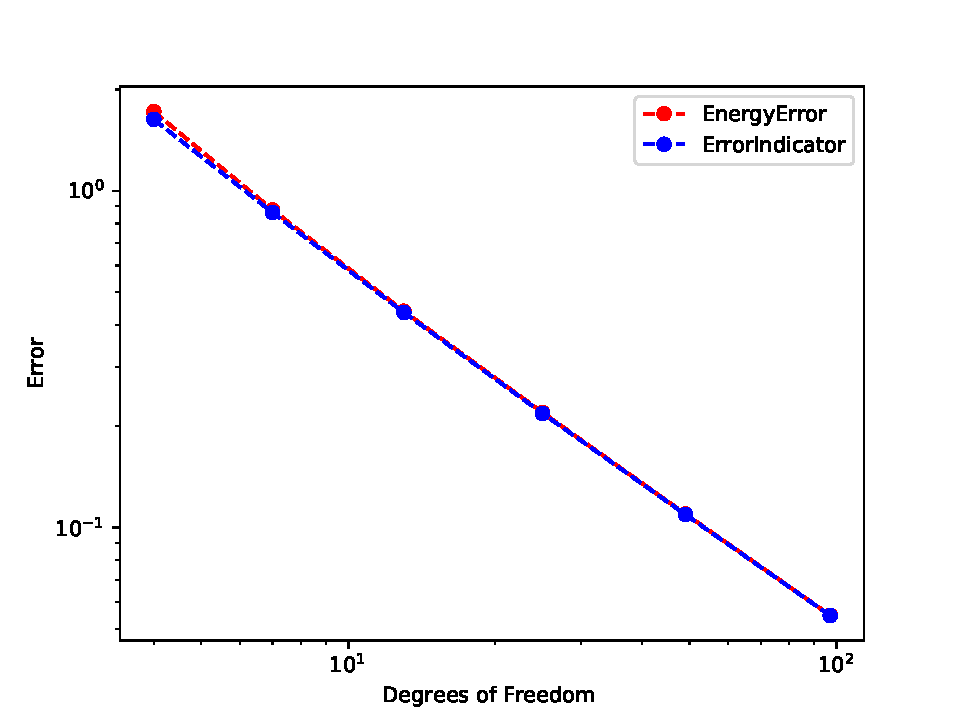
\includegraphics[width=0.5\textwidth]{IndicatorPDE1.pdf}
   
 \label{fig:IndicatorPDE1}
\end{figure}

\begin{center}
  \begin{tabular}{r|cccccc}  \label{table:IndicatorPDE2}
    $Mesh$   & DOGs & $\|u-u_h\|_{a(0,1)}$ & $\|\eta\|$  \\ \hline
    $1$ & $4$ & 0.29131 &  0.108467   \\
    $2$ & $7$ & 0.074447 &  0.0201663   \\
    $3$ & $13$ & 0.0229916 & 0.0135003   \\
	$4$ & $25$ & 0.00855775 &  0.00718688  \\
    $5$ & $49$ & 0.00381445 &  0.00363495   \\
    $6$ & $97$ & 0.00184453 &  0.00182187  \\
  \end{tabular}
\end{center}



\begin{figure}[h]
   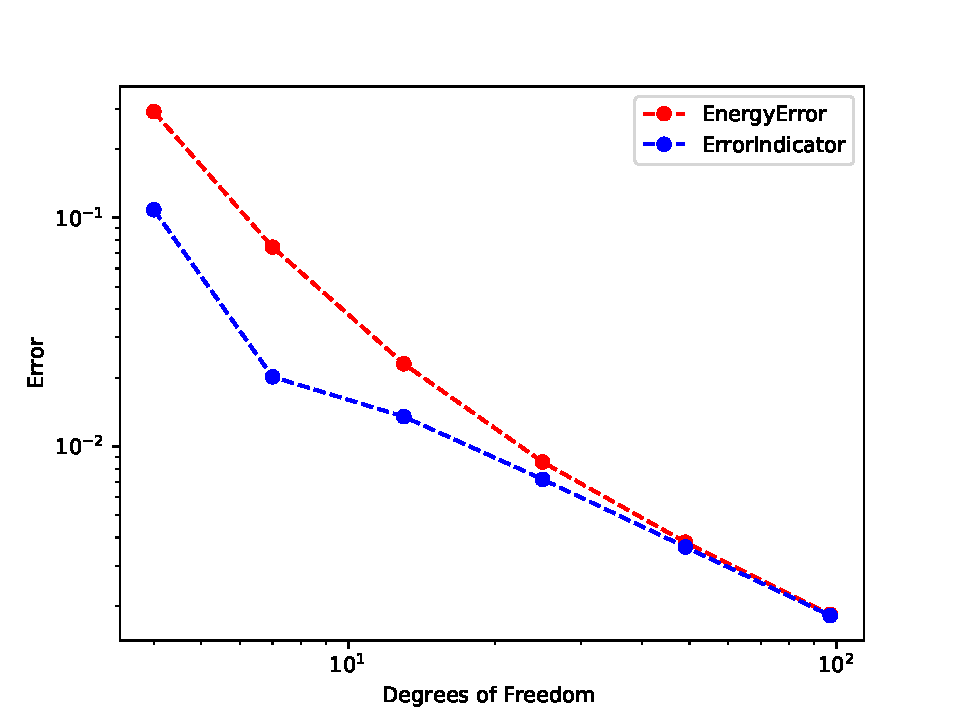
\includegraphics[width=0.5\textwidth]{IndicatorPDE2.pdf}
   
 \label{fig:IndicatorPDE1}
\end{figure}

\subsection{Implementation} \label{subsubsec:KK Implementation}

To make the most use of our existing member functions in the SpaceMesh class we should make sure our gradient recovery vector match the space nodes. This will allow the interpolant to be completely defined by the new vector and a reference to a grid. This means that the first and last point though should be defined on the boundary. In practise this means hard coding an interpolant over the first and last element and taking its value at the boundary.

\begin{lstlisting}[language=C++]
void GeneralHeat::GradientRecoveryFunction( SpaceMesh& relevantMesh,
       std::vector<double>& gradvec, std::vector<double>& gradrecovery ) {
    	
    	//(x_0, y_0) (x_1, y_1) define the line segment to be hard coded
    double x_0 = 0.5*(relevantMesh.ReadSpaceNode(1)+
    				relevantMesh.ReadSpaceNode(0));
    double y_0 = gradvec.at(0);
    double x_1 = relevantMesh.ReadSpaceNode(1);
    double y_1 = 0.5*(gradvec.at(1)+gradvec.at(0));

    gradrecovery.push_back(y_0+(relevantMesh.ReadSpaceNode(0)-
    						x_0)*(y_1-y_0)/(x_1-x_0));
		
		//take the midpoint of the two gradients where undefined
    for(int i = 0; i<relevantMesh.meshsize()-1; i++)
    {
        gradrecovery.push_back(0.5*(gradvec.at(i)+gradvec.at(i+1)));
    }
		
		//the hardcoding needs to happen on both sides
    x_0 = relevantMesh.ReadSpaceNode(mpsmesh.meshsize()-1);
    y_0 = gradrecovery.back();
    x_1 = 0.5*(relevantMesh.ReadSpaceNode(relevantMesh.meshsize())			   
    +relevantMesh.ReadSpaceNode(relevantMesh.meshsize()-1));
    y_1 = gradvec.back();

    gradrecovery.push_back(y_0+
    (mpsmesh.ReadSpaceNode(mpsmesh.meshsize())-x_0)*(y_1-y_0)/(x_1-x_0));
}

\end{lstlisting}



\newpage

\section{Design of Adaptive Algorithms} \label{sec:Adaptive}



\subsubsection{Space Adaptivity} \label{subsubsec:KK Implementation}

\subsection{Results} \label{subsec:results3}

\subsection{Time Adaptivity} \label{subsubsec:Time Adaptivity}

\newpage

\section{Some Numerical Examples} \label{sec:Examples}

\newpage


\section{Conclusions} \label{sec:conclusions}

Further help on \LaTeX\ can be found easily on the internet. The \LaTeX\
wikibook\footnote{\tt http://en.wikibooks.org/wiki/LaTeX} contains a lot.
For instance you would find there how to type theorems and proofs nicely.
Or how to include source code written in some programming language like
matlab. There are long lists available with all sorts of common
mathematical symbols like $\xi$, $\nabla$, $\infty$, $\log$, $\iff$, etc.

\newpage

\appendix

\section{Raw data} \label{app:rawdata}



\section{Calculations for section \ref{sec:my1}} \label{app:calculations}

In this appendix we verify equation \eqref{eq:myeq1}.

\newpage

	\bibliography{References}
	\bibliographystyle{plain}

\end{document}
